 %!TEX root = jsba_main.tex
% Method section

\section{Methods}
\label{sec:meth}
 
 \begin{enumerate}
     \item show how your choice of design and research method is suited to answering your research question(s)
     \item demonstrate that you have given due consideration to the validity and reliability of your chosen method
     \item by “showing” instead of “telling”, you demonstrate that you have understood the practical meaning of these concepts
     \item Show the reader what you have done in your study, and explain why. 
     \begin{enumerate}
         \item How did you collect the data? 
         \item Which options became available through your chosen approach?
         \item What were your working conditions? 
         \item What considerations did you have to balance?
     \end{enumerate}
    \item Tell the reader what you did to increase the validity of your research. 
    \begin{enumerate}
        \item E.g., what can you say about the reliability in data collection? 
        \item How do you know that you have actually investigated what you intended to investigate? 
        \item What conclusions can be drawn on this basis? 
        \item Which conclusions are certain and which are more tentative?
        \item Can your results be applied in other areas? Can you generalise? If so, why? If not, why not?
    \end{enumerate}
    \item You should aim to describe weaknesses as well as strengths. An excellent thesis distinguishes itself by defending – and at the same time criticising – the choices made.
 \end{enumerate}
 
\todo[inline]{Maybe switch following section to implementation chapter instead of methdods}

\subsection{Apache Ignite}
\label{sec:meth_ign}

\citetalias{Ignite} is desribed as a "memory-centric distributed database, caching, and processing platform for transactional, analytical, and streaming
workloads delivering in-memory speeds at petabyte scale" (\citetalias{Ignite}, see also \url{https://apacheignite.readme.io/docs} for the full
documentation).
Its main features are distributed in-memory storage as well as optionally persistent storage of data on the disk that can be treated as a distributed, join
supporting SQL database or as a distributed key-value in-memory data grid. There are a lot more features provided by \citetalias{Ignite} that are not of
relevance here and will be left out because of that reason, thus, in the following there will be a focus on the distributed SQL database part.
Furthermore, the implementation will be based on a pure in-memory storage where all the data will be stored entirely in the RAM without any persistent 
storage of the data due to performance issues. The of \citetalias{Ignite} provided SQL-capable in-memory DDB instances can be spread across the network via 
a set of interconnected Ignite nodes that form a so-called \emph{cluster}. Each node of the cluster can be hosted by a different machine in a Java Virtual 
Machine (JVM), but there can be multiple nodes on the same machine, too. A node can be either a server node, which is responsible for storing and 
processing data, or a client node that is able to connect remotely to the cluster and compute or query from the client side. Figure~\ref{fig:ign_cluster} 
shows a sample cluster consisting of 6 server nodes which are responsible for computations and storing data. This servers can be accessed remotely from 
clients that can connect to the cluster via an programming language API (e.g. Java), via a JDBC or ODBC connection or via a REST-API (see documentation
for details).

\begin{figure}[h]
    \centering
    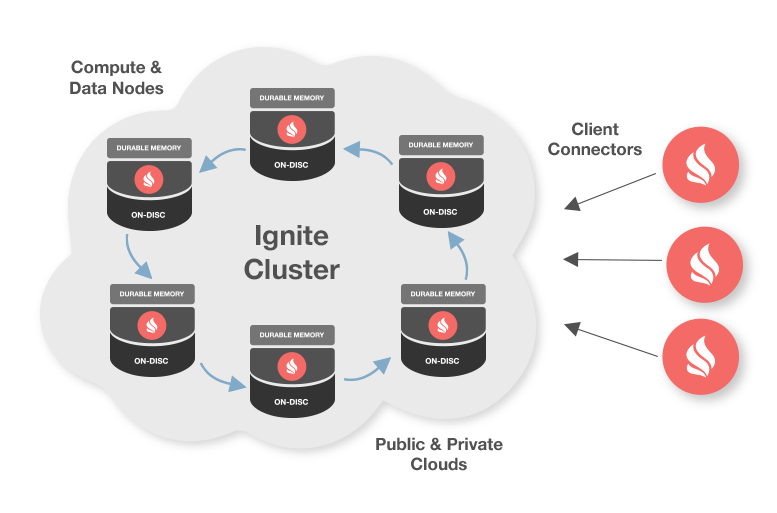
\includegraphics[width=0.75\textwidth,keepaspectratio=true]{img/9287d3c-ignite-deploy.png}
    \caption{Ignite Cluster. Source: \protect\url{https://apacheignite.readme.io/docs/clustering} (Accessed 16th Feb 2019)}
    \label{fig:ign_cluster}
\end{figure}


\subsubsection{Partitioning and Replication}
\label{sec:meth_ign_panre}
The server nodes of an Ignite cluster store some certain data of the whole data set depending on the fragmentation (partitioning, cf.
Section~\ref{sec:theo_ddb_frag}) and replication (cf. Section~\ref{sec:theo_ddb_repl}). The fragmentation and replication is always defined for relations,
i.e. the tables of the relational DDB. For example, under full replication each server would store the total data of the relation and in the partitioned 
mode the relation is partitioned and each server is then responsible for only a subset of the data. It is also possible to have partitioning and replication
at the same time if the partitions of the data are stored on more than one server such that each partition of the data is stored on one server as primary
partition and on the other servers as backup copies for higher availability and data resiliency in case of server node failures. In replicated mode, a
balancing of the data load is achieved by a partitioning of the data of the relation with hash functions into subsets of nearly equal size that are
dispersed equally among all nodes of the cluster to exploit as much memory as possible on all nodes. However, even more memory is available if there 
is no replication of the data in form of redundant copies that would consume additional parts of the total available memory. 

The partitioning is always a horizontal fragmentation of the data but the way how this is computed is only syntactically defined with hash functions, thus,
there are no explicit selection conditions on a certain attribute of the relation that represent a horizontal fragment as described in the
Section~\ref{sec:theo_ddb_frag}, and the assignment of tuples to the partitions of the relation they belong to is done rather arbitrarily. The only way to
influence and change this assignment of a tuple to a partition is via an affinity function, which is explained in the following section.



\subsubsection{Affinity Collocation and Distributed Joins}
\label{sec:meth_ign_affc}

One important concept of \citetalias{Ignite} is the collocation of data with data that corresponds to the concept of a derived horizontal fragmentation 
(cf. Section~\ref{sec:theo_ddb_frag}). Hereby, data that is accessed together, e.g. because it is joined via a common attribute or a foreign key reference,
is also stored together on the same server which improves the data locality~\citep{Wiese2014} and allows for collocated distributed joins that benefit from
this improvement in the data locality as the costly data transfer of data, which is required to obtain an answer to a query, across the network is 
avoided. This \emph{affinity collocation} is internally defined for the key-value store underlying the relational SQL database and restricts its usage to 
a single affinity key definition per relation. With this restriction, there can not be a collocation of three or more relations that could be joined via a 
chain of join conditions where the joining attributes, that would form a possible affinity key, are different. An affinity key be the same as the primary 
key of the relation or an attribute of a composite primary key.

Joins between partitioned relations require for collocation of the data that is about to be joined, otherwise a non-collocated distributed join has to be
performed or the result set will be incomplete as the non-collocated parts of the data can not be joined locally by the nodes. If all the joined relations
in the SQL query are collocated, the query can be evaluated locally by each node, because all the data they need to compute a correct result set regarding 
their portion of the whole data in the cluster is available, i.e. stored by themselves. The query execution for this case is depicted in
Figure~\ref{fig:ign_collocated} where the query $Q$ is sent from the client to each server node which executes the query $Q$ locally 
and returns the result set $R_i$ to the query according to its stored data set. The final result set is the accumulation of the result sets $R_1+R_2+R_3$
which is meant as union of the result sets. This computation of the result set as union of locally obtained result sets is very similar to the localization
program \cite[p.~199]{Ozsu1991} as introduced in Section~\ref{sec:theo_dqp_decomp} where the union of all the fragments of certain relations is used to
rewrite the query in order to execute it in a distributed fashion.  
\begin{figure}[ht]
    \centering
    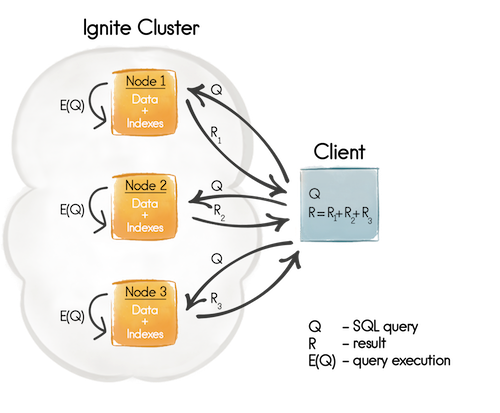
\includegraphics[width=0.6\textwidth,keepaspectratio=true]{img/2af89cf-Collocated_sql_queries.png}
    \caption{Collocated SQL Query. Source: Picture 1, \protect\url{https://apacheignite-sql.readme.io/docs/distributed-joins} (Accessed 16th Feb 2019)}
    \label{fig:ign_collocated}
\end{figure}

On the other side, non-collocated joins require for additional communication and data transfer between the nodes of the cluster as the data, that is needed
for a join or another computation, is not locally present, thus, the nodes have to sent requests for the data to other nodes to complete their result set 
computations appropriately. This additional data transfer implies a bad efficiency of query execution as it depends on the transmission duration of
probably bigger data sets between the nodes. Furthermore, this causes additional load on the network that can decrease the performance of other tasks or
operations. The query execution of a non-collocated, distributed query is sketched in Figure~\ref{fig:ign_noncoll}. 
\begin{figure}[ht]
    \centering
    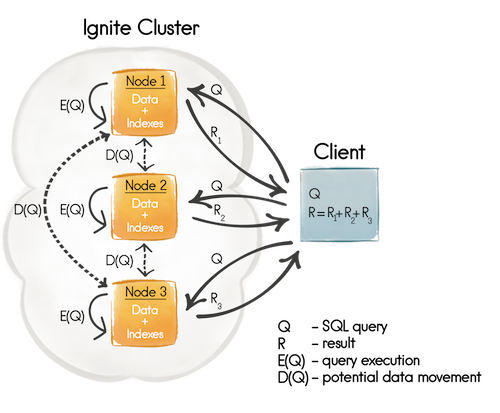
\includegraphics[width=0.6\textwidth,keepaspectratio=true]{img/95f09db-Non_collocated_sql_queries.png}
    \caption{Non-Collocated SQL Query. Source: Picture 2, \protect\url{https://apacheignite-sql.readme.io/docs/distributed-joins} (Accessed 16th Feb 2019)}
    \label{fig:ign_noncoll}
\end{figure}
 
In comparison to Figure~\ref{fig:ign_collocated}, the additional data transfer, that might occur in relation to the non-collocated query, is depicted as
potential data movement $D(Q)$ in a peer-to-peer fashion between all pairs of nodes. However, the data request of a node can be sent as a unicast request 
to a certain node of the cluster (peer-to-peer communication) or as a broadcast request to all other nodes. This decision depends on whether the 
requesting node can identify the exact location of the data, i.e. if it is a join on a primary or affinity key, or if it has to request the missing data
from all other nodes otherwise.

 
\subsection{Clustering-based Fragmentation}
\label{sec:meth_cbfr}

\subsection{Similarity-based Query Answering}
\label{sec:meth_sbqa}